\scanpage{55}
Nous allons aussi déterminer les groupes modulaires $\Gamma$ et $\Gamma^!$ correspondant à ces six cas :
\margin{MD-graphes \unsure{maximaux|minimaux} (dim mod. nulle), de dim. modulaire ambiante $\leq2$}
\figure{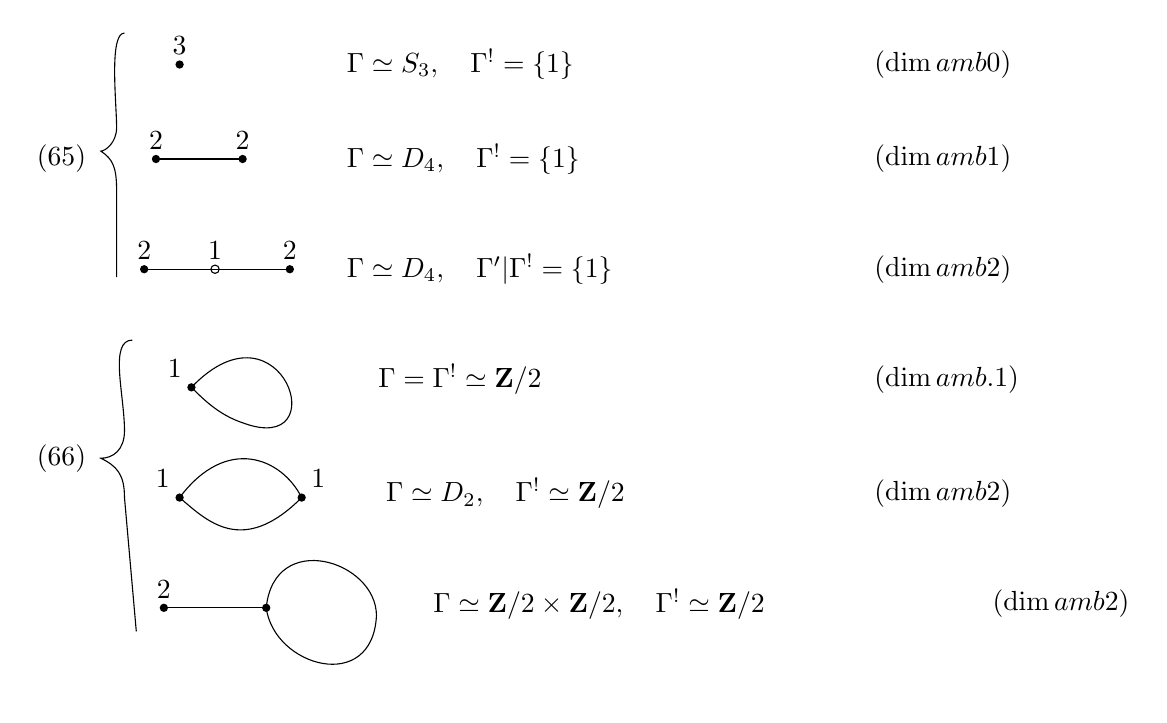
\begin{tikzpicture}[x=1cm,y=1cm]
\node at (-1.5,-1.2) {$(65)$};\draw (-.7,.4) .. controls (-.9,.4) and (-.8,-.5) .. (-.8,-.8) .. controls (-.8,-1) and (-.95,-1.1) .. (-1,-1.1) .. controls (-.85,-1.2) and (-.8,-1.3) .. (-.8,-1.6) -- (-.8,-2.7);
\fill (0,0) circle(1.5pt);\node[above] at (0,0) {$3$};\node[right] at (2,0) {$\Gamma\simeq\unsure{\mathfrak S}_3,\quad\Gamma^!=\{1\}$};\node[right] at (8.7,0) {$(\dim\operatorname{amb}0)$};
\draw (-.3,-1.2)--(.8,-1.2);\fill (-.3,-1.2) circle(1.5pt);\fill (.8,-1.2) circle(1.5pt);\node[above] at (-.3,-1.2) {$2$};\node[above] at (.8,-1.2) {$2$};\node[right] at (2,-1.2) {$\Gamma\simeq D_4,\quad\Gamma^!=\{1\}$};\node[right] at (8.7,-1.2) {$(\dim\operatorname{amb}1)$};
\draw (-.45,-2.6)--(1.4,-2.6);\fill (-.45,-2.6) circle(1.5pt);\draw (.45,-2.6) circle(1.5pt);\fill (1.4,-2.6) circle(1.5pt);\node[above] at (-.45,-2.6) {$2$};\node[above] at (.45,-2.6) {$1$};\node[above] at (1.4,-2.6) {$2$};\node[right] at (2,-2.6) {$\Gamma\simeq D_4,\quad\unsure{\Gamma'|\Gamma^!}=\{1\}$};\node[right] at (8.7,-2.6) {$(\dim\operatorname{amb}2)$};
\node at (-1.5,-5) {$(66)$};\draw (-.6,-3.5) .. controls (-.9,-3.5) and (-.7,-4.2) .. (-.7,-4.65) .. controls (-.7,-4.9) and (-.85,-5) .. (-1,-5) .. controls (-.8,-5.1) and (-.7,-5.2) .. (-.7,-5.5) -- (-.55,-7.2);
\draw (.15,-4.1) .. controls (1.3,-2.9) and (2,-5) .. (.8,-4.55) .. controls (.5,-4.45) and (.3,-4.25) .. (.15,-4.1);\fill (.15,-4.1) circle(1.5pt);\node[above left] at (.15,-4.1) {$1$};\node[right] at (2.4,-4) {$\Gamma=\Gamma^!\simeq\mathbf Z/2$};\node[right] at (8.7,-4) {$(\dim\operatorname{amb}.1)$};
\draw (0,-5.5) .. controls (.6,-4.7) and (1.3,-5) .. (1.55,-5.5) .. controls (.8,-6.25) and (.35,-5.8) .. (0,-5.5);\fill (0,-5.5) circle(1.5pt);\fill (1.55,-5.5) circle(1.5pt);\node[above left] at (0,-5.5) {$1$};\node[above right] at (1.55,-5.5) {$1$};\node[right] at (2.5,-5.45) {$\Gamma\simeq D_2,\quad\Gamma^!\simeq\mathbf Z/2$};\node[right] at (8.7,-5.45) {$(\dim\operatorname{amb}2)$};
\draw (-.2,-6.9)--(1.1,-6.9);\draw (1.1,-6.9) .. controls (1.2,-5.9) and (2.5,-6.3) .. (2.5,-7.0) .. controls (2.45,-8) and (1.2,-7.65) .. (1.1,-6.9);\fill (-.2,-6.9) circle(1.5pt);\fill (1.1,-6.9) circle(1.5pt);\node[above] at (-.2,-6.9) {$2$};\node[right] at (3.1,-6.85) {$\Gamma\simeq\mathbf Z/2\times\mathbf Z/2,\quad\Gamma^!\simeq\mathbf Z/2$};\node[right] at (10.2,-6.85) {$(\dim\operatorname{amb}2)$};
\end{tikzpicture}}
Notons que pour un \inserted{MD-}graphe $G$ de dim modulaire nulle, si $(\mathcal X,I_S)$ est une \inserted{MD-}courbe \deleted{\unsure{à}} $G$-épinglée sur une base $S$ connexe, alors le groupe des autom. de $(\mathcal X,I_S)$ (où on a oublié l'épinglage) est can. isom. à $\Gamma$, et \deleted{alors} le \deleted{$\unsure{X,I}$} sous-groupe qui induit l'identité sur $I_S$ est can. isom. à $\Gamma^!$.
\margin{54}
